\section{Estimating wallet geographical position}
The goal of this project is to investigate whether there is some locality in Ripple transactions. After having a brief overview of how the Ripple network operates we can now start to explore different techniques to estimate wallets geographical positions.

\subsection{Finding the IP of wallets}
Nodes are the backbone of the Ripple Network. Our first focus was to dig into the possibilities that nodes could give us. This section describes unsuccessful techniques, readers in a rush can jump to section 3.2

\subsubsection{Ripple crawler}
We found a crawler\cite{crawler} that crawl Ripple nodes, and could give us geographical positions. At first, it seemed a good idea that could give us estimates of the positions of the wallets. However, as mentioned in the Ripple background section, the wallets and the nodes are not linked directly. This crawler finally turns out to be useless since it could only give us information about nodes and not on wallets.

\subsubsection{Connect to existing nodes}
Another angle to tackle the problem was to find out if clients have preferred nodes they connect to. Maybe the closest ones ? To explore this idea, we found the list of all nodes and their IP address using the Ripple Data API\cite{data-api}. We used a Python implementation Data API calls to query the Ripple Data API to get all nodes IP and then get their URL. Then for all those nodes, we tried to connect to them on port 51235 (most used port) to see if we could access the Ripple Ledger. It turns out that we were not able to connect to any nodes. It seems that users that run a node use it as their own copy of the ledger, and so don't have to rely on someone else. The only way we managed to connect to a node and query the ledger was to connect to the public Ripple node maintained by Ripple Inc. 

\subsubsection{Running our own node}
While trying to estimate wallet position, we thought about running nodes in various locations. Since we know nodes are responsible for propagating transactions, having several nodes in several parts of the world could enable us to hear transactions and tell that the sender is probably closer to the location of the first node who learns about the transactions. The problem is that it does not seems that in the peer protocol nodes connect to other nodes that are close to them. So the idea that transactions propagate along with geographic positions does not seem to fit here.

However, if we could get client connection to our nodes to send their transaction then we could know thanks to IP address position of the actual sender of the transactions. But how to get users sending their transactions to us? The only way would be to advertise our node since users can choose freely the node they want to use to send their transaction. We believe that we would get only a few users connection to our servers if any. In addition, we looked at the source code of some popular Ripple clients and from what we could learn it seems those clients connect to the public nodes maintained by Ripple. This promising idea finally turned out to be left out, as most of the users go through the same node to propagate their transactions then we would probably retrieve any information from running our own nodes.

\subsection{Running a gateway}
Gateways are highly connected wallets in the Ripple network, they are the door between the Ripple network and the real world. A new wallet in the Ripple network can create a credit link with a gateway then send (in the real world) some money to this gateway and then the user will have this credit available on the link with the gateway. The idea is that when a user goes on the gateway platform, creates a wallet and send money to a gateway, then the gateways are able to link wallet identifiers to a real-world person with their location thanks to either the IP address or either the postal address (usually gateways ask it due to regulations). Hence our first idea was then to look at whether it was easy to run a gateway and have clients connecting to us. It turns out the Ripple documentation\cite{runGateway} gives the steps to run a gateway but due to the complexity and costs constraints we abandoned the idea, it is left as further work.

\subsection{Nodes positions}
As explained above, the Ripple Data API\cite{data-api} enables us to know all nodes and their IP. We can then process the IP addresses obtained and map each node to a country.

\begin{wrapfigure}[9]{l}{0.4\textwidth}
    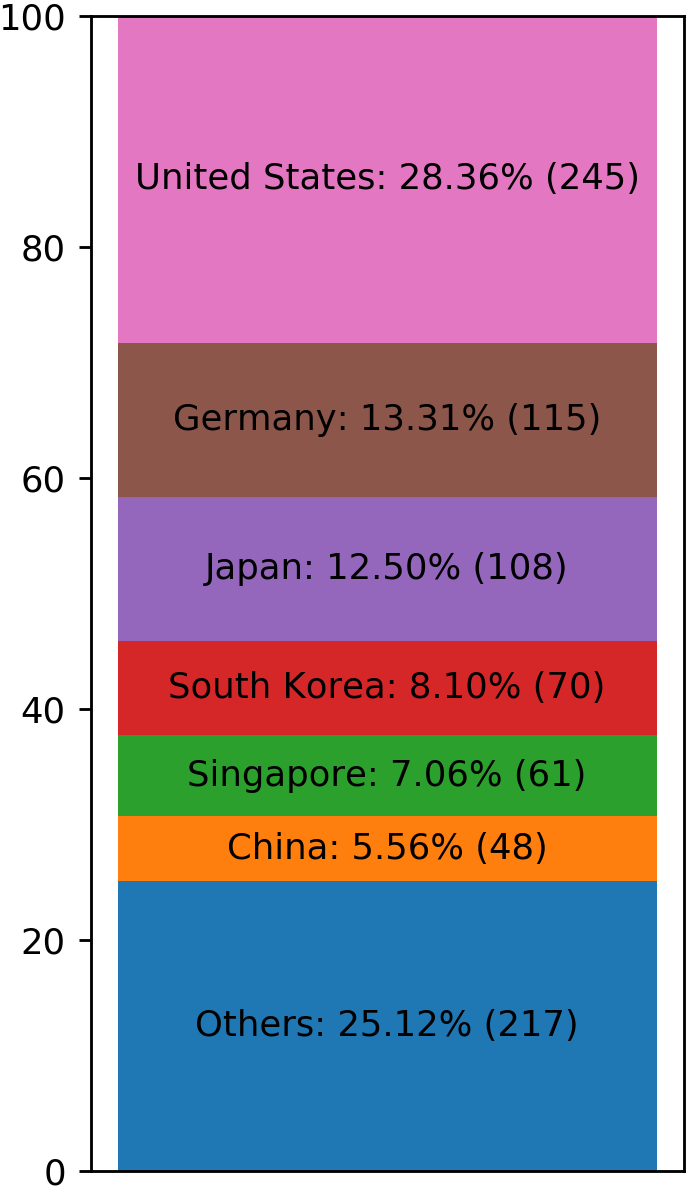
\includegraphics[width = 0.35\textwidth,keepaspectratio]{repartiton_of_nodes.png}
    \caption{Repartition of Ripple nodes}
    \label{fig:repartition}
\end{wrapfigure}

Figure \ref{fig:repartition} on the left shows the repartition of the 868 nodes we were able to locate over 1018 that are known to the API. For each candidate country, we show the percentage and in parenthesis the actual number of nodes situated in the country. We regrouped all countries that count for less than 5\% each in the 'Others' category. We used a stacked bar chart because it helps to visualize proportion and compare values.

We see that the country that has the most node is the United States then comes Germany and Japan. Together they represent more than 50\% of all nodes. 
\vspace{\baselineskip}

We want to see if the number of nodes in a country is correlated to how this country's currency is used in the Ripple ledger.

\begin{figure}[h!]
    \centering
    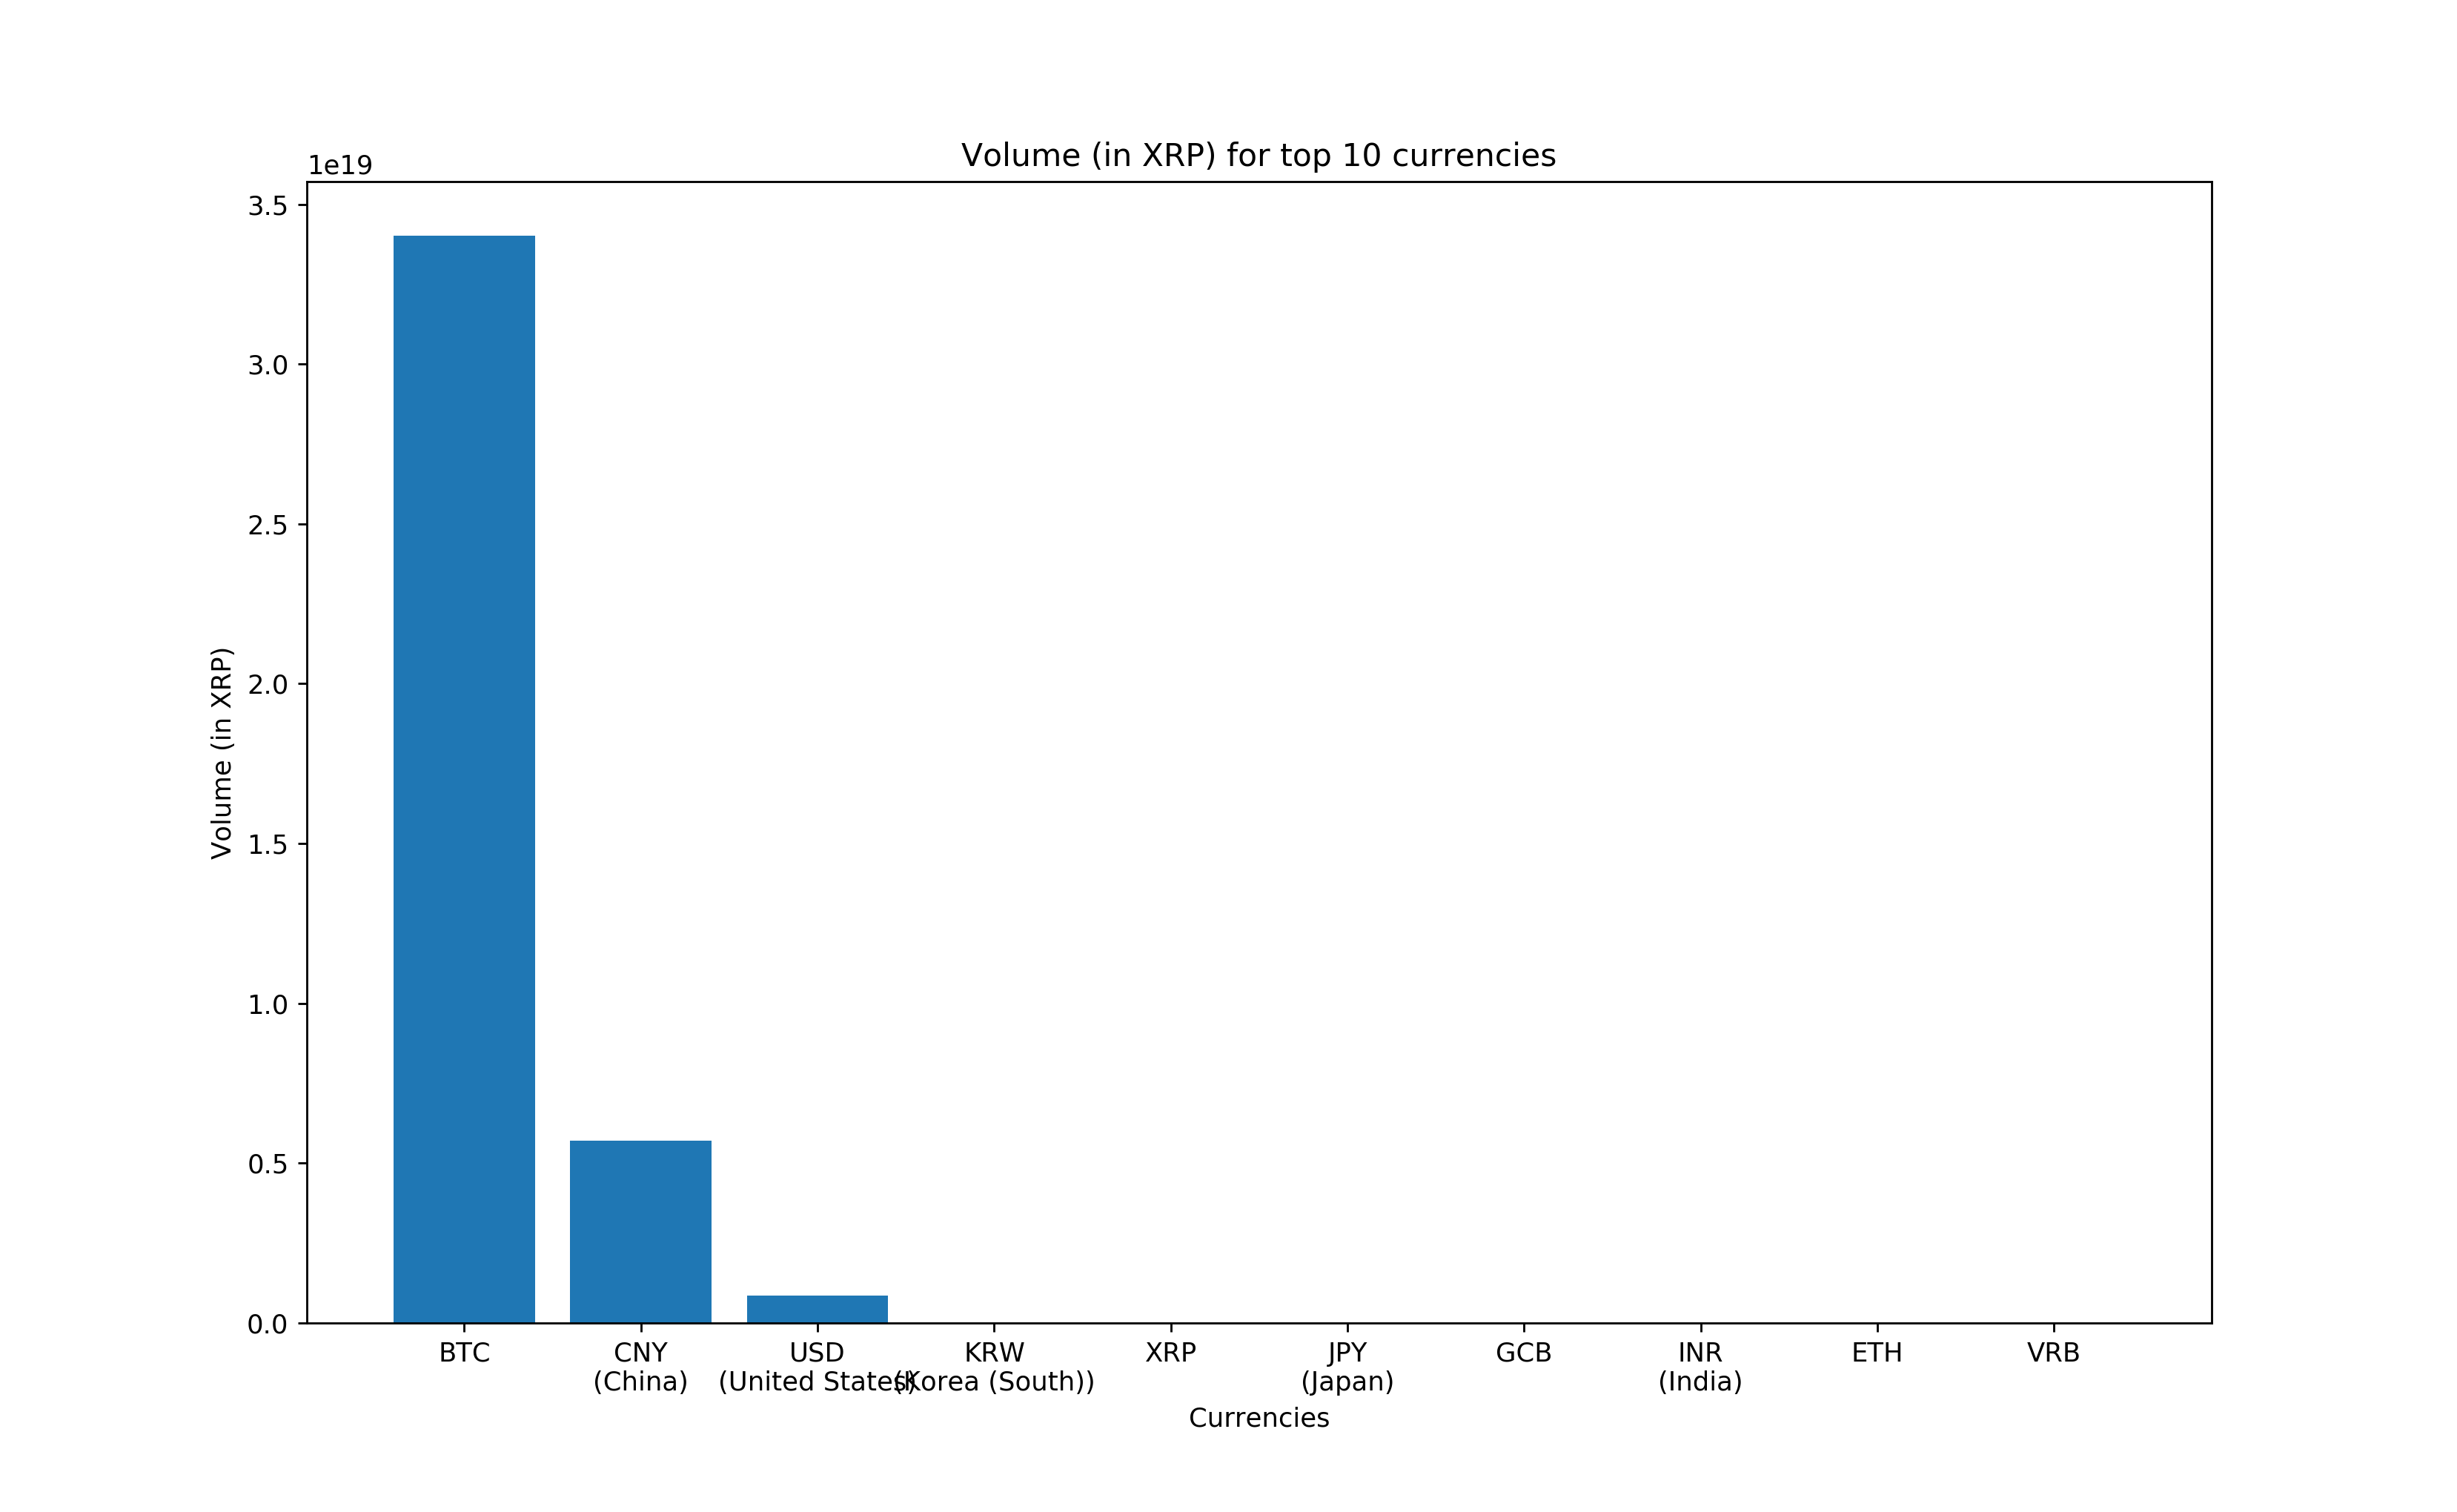
\includegraphics[width = 0.95\linewidth]{top_10_currencies_in_volume_in_XRP.png}
    \caption{Top 10 currencies in XRP volume}
    \label{fig:volume}
\end{figure}

Figure \ref{fig:volume} shows the volume, in XRP, for the 10 currencies with the highest volumes. We chose to represent the result as a bar chart to ease the comparison between currencies. We see that CNY have a much higher volume that USD but on Figure \ref{fig:repartition} we saw that the United States had more nodes. We can also say that Japan has more nodes than South Korea but that KRW has higher volume. So our assumption that we could extract some locality information from the position of the nodes does not seem to fit here since the number of nodes in a country does not reflect how this country's currency is used in the Ripple Network.

\subsection{Using transactions data}
Let's try a different approach to gain further information about the localization of Ripple transactions. What could be better than looking directly at the actual transactions data? The data we used was provided by Pedro Moreno-Sanchez who is one of the publishers of the paper Mind Your Credit: Assessing the Health of the Ripple Credit Network\cite{MindYourCredit} which motivated us for this semester project. We have 3 files with transactions data, one that contains transactions from January 2017 to August 2017, one that has transactions from 2013 to 2016 and another file with some missing transactions from 2013 to 2016.

In the next subsections we want to look at path in the Ripple network and sender/receiver currency pairs, the file with data from 2013 to 2016 was not really useful for this step because we didn't have any information about the path of transactions and it shows contains only the receiver's currency not the sender's.

We also did a little bit of cleaning on the files that were usable because for some transaction the sender's currency was missing so we had to infer it from the path.

\subsubsection{Looking at credit links}
For the reader that will look at the Jupyter notebooks, notice that credit links are called trust lines in the Ripple Data API\cite{data-api}. Thanks to this API and our additional work, we could recover all credit links for the wallets that appear in our transactions data. We then computed a few statistics on those credit links.

We have that 43.34\% of wallets have at least one credit link. Over the wallets that have at least one credit link 69.59\% of them have one with a gateway (that is 30.17 \% of all wallets). Overall credit links, 69.24\% of them are with gateways.

It seems that gateways play an important role in credit links. Can we get any information from those credit links to help in our goal of localizing transactions?

As we explained before, each credit link is associated with a currency. We looked for each wallet how many different currencies link them to gateways. For the wallets that have credit links with gateways, we have that 75.95\% of them that are linked to gateways via only 1 currency and we have 19.94\% that are connected via only 2 currencies. From those results, it seems that wallets tend to keep a small number of currencies on links with gateways. Why wallets would behave like this? One hypothesis we made to answer this question was that wallets tend to use their local currency in the Ripple network. However, this assumption can't be easily verifiable and only a few of all wallets are concerned by this hypothesis.

We now present another look at credit links where we looked at the currencies that linked the sender and gateway on the first hop of a transaction (and respectively the gateway and the receiver on the last hop). A gateway is a first hop (respectively a last hop) if it is the first wallet after the sender on the path from sender to receiver (respectively the last wallet before the receiver).

\begin{figure}[h!]
  \makebox[\textwidth][c]{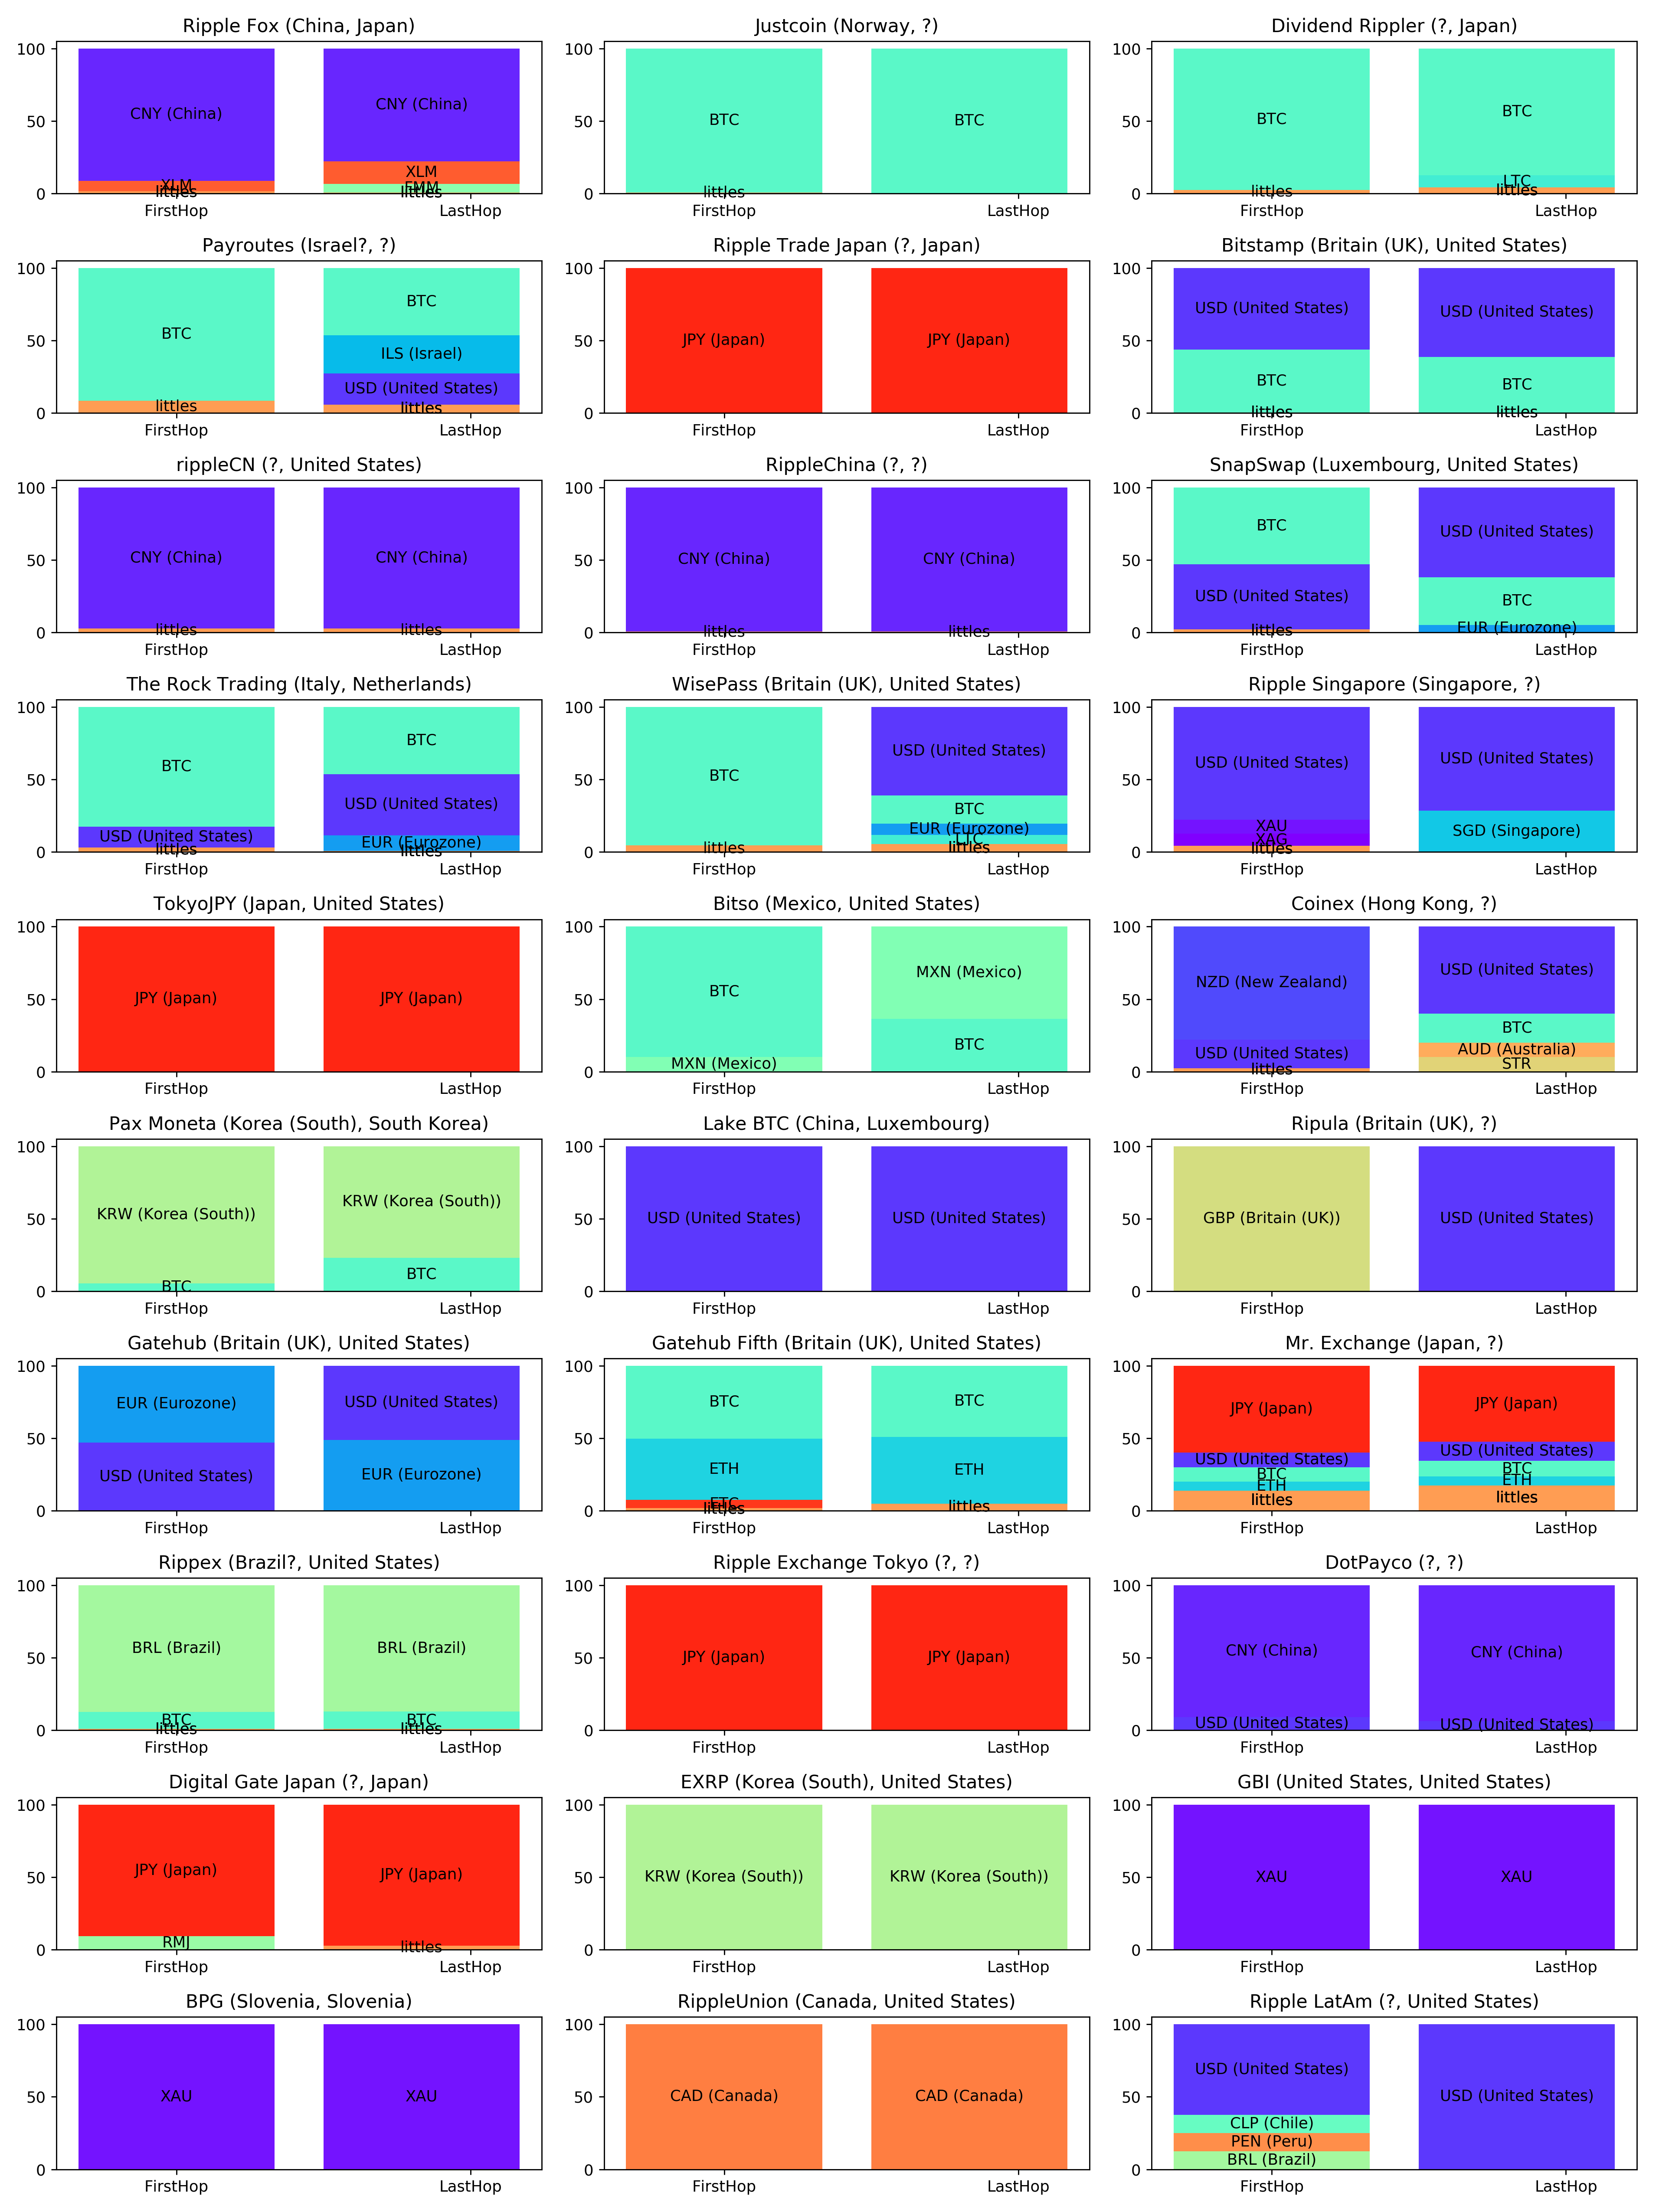
\includegraphics[width=1.1\textwidth]{first_last_hop_currencies_per_gateways.png}}
  \caption{Currency of transaction for first and last hop per gateway}
    \label{fig:first_lap_hop_per_gateway}
\end{figure}

The stacked-bars in Figure \ref{fig:first_lap_hop_per_gateway} show as a percentage the currencies of the link where the gateway appears as first or last hop. Each subgraph represents a gateway, we distinguish the first hop on the left and last hop on the right. On top of each subgraph, you can see the name of the gateway along with a parenthesis with two countries. The first country is the supposed fiscal location of the gateway found on this website\cite{wipple} and the second country is the where the gateway's servers are situated. We got the server's location thanks to the Ripple Data API\cite{data-api} that could give us the domain of the gateways then from those domains we got the corresponding IP addresses and mapped them to a country. What is important to look at here is the colors, each color corresponds to a currency.

On this graph, we can see that most of the subgraph contains one or two colors. This means that gateway seems to be active on at most 2 preferred currencies. We can also note that there seems to be a correlation on the location of the gateway and its currencies. For example, the first one 'Ripple Fox', supposedly situated in China, seems to process mainly CNY which is the Chinese currency. The same applies to Ripple Trade Japan where the servers of this gateway are situated in Japan and it processes only JPY the currency of Japan. 

It seems that gateways tend to specialize. We know they are financial institutions that are looking for profit, so if there must be an explanation as to why they seem to stay local. We think that people try to connect to the gateway that will offer their local currency and that hence that is situated the closest to them. Again we don't know if this is true, but otherwise, gateways will tend to offers more and more currencies to attract more clients in order to have higher profits.

\subsubsection{Evolution of credit links}
Following up with the results we obtained on credit links, we wanted to investigate the behavior of those lasts over time. The previous analysis was just over the credit links we could get from the Ripple Data API\cite{data-api} and does not reveal an evolution in time. To palliate this problem we looked at transaction paths which use credit links. We only treated transactions from 2017 because it was the year with the most information about transaction paths. We computed for each currency and for each month the wallets appearing as first or last hops. For those wallets, we then compute the total volume and number of transactions routed through them per month. We only showed a wallet if it had a month where the amount was significant enough (1\% of the biggest value over the year). We plotted the results for CNY, JPY, USD, and EUR the 4 top currencies in terms of the number of transactions. All graphs are visible on the Github repo\cite{repo}. We show the ones for USD in this report, as they are the most interesting. 

\begin{figure}[h!]
  \makebox[\textwidth][c]{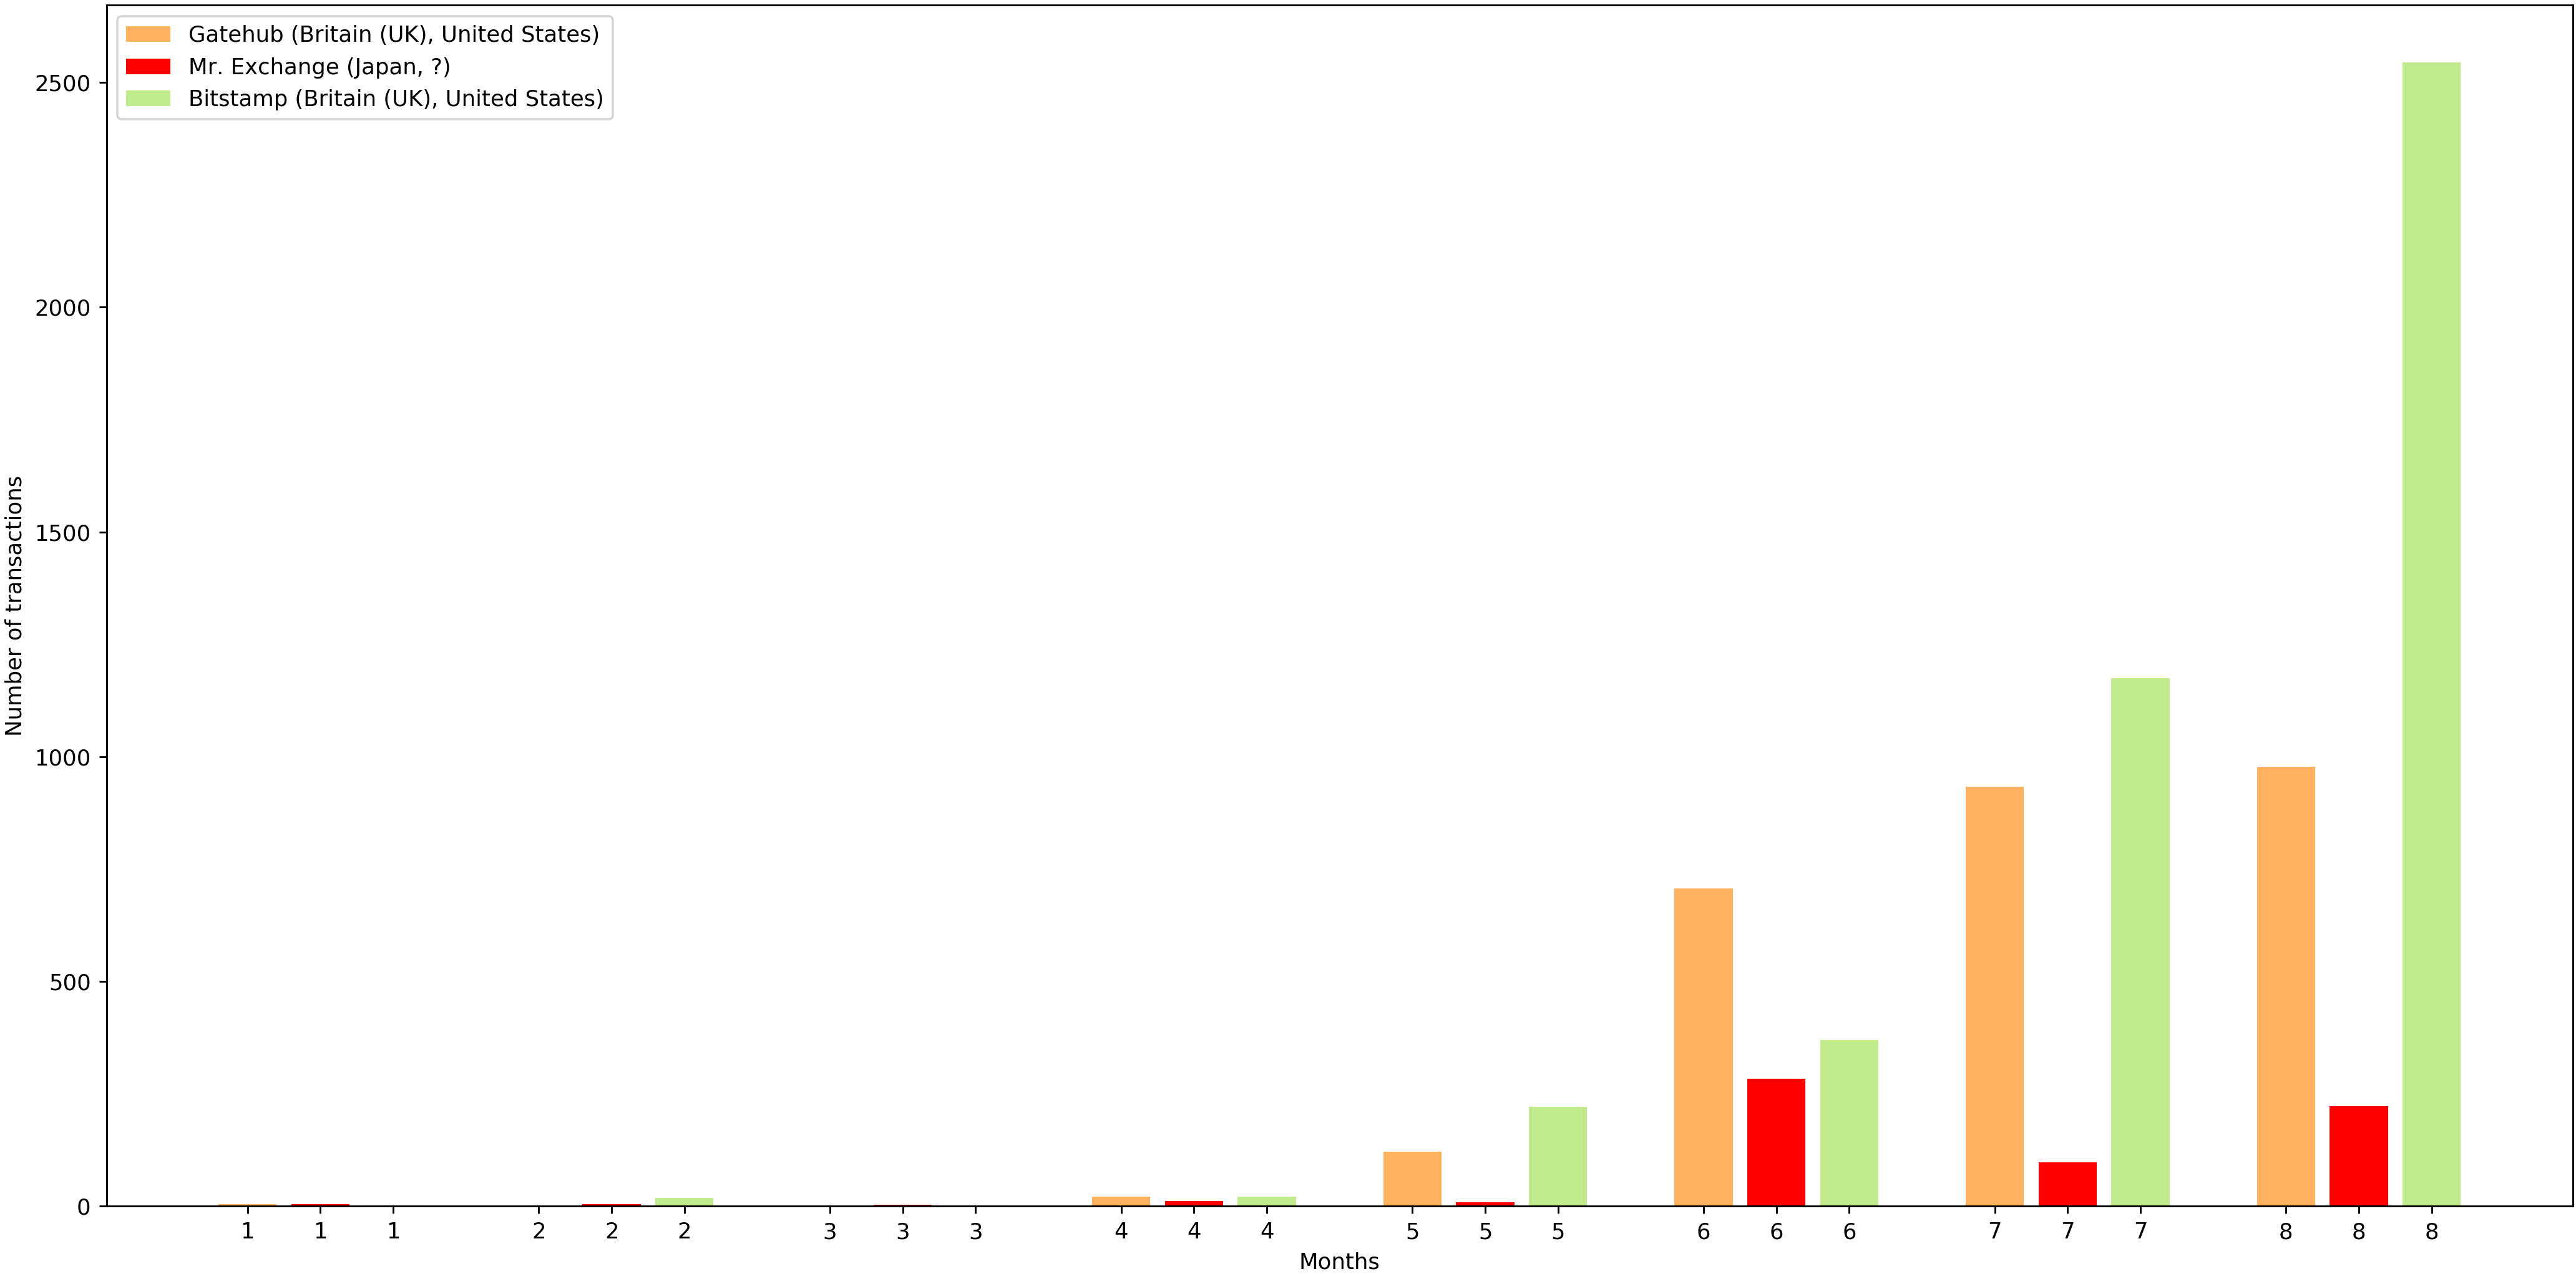
\includegraphics[width=1.375\textwidth]{number_of_transactions_processed_by_gateways_as_first_hop_for_USD_in_2017_per_month.png}}
  \caption{Number of transactions routed trough wallets as first hop for USD in 2017}
  \label{fig:first_hop_USD_nb_txns}
\end{figure}

\begin{figure}[h!]
  \makebox[\textwidth][c]{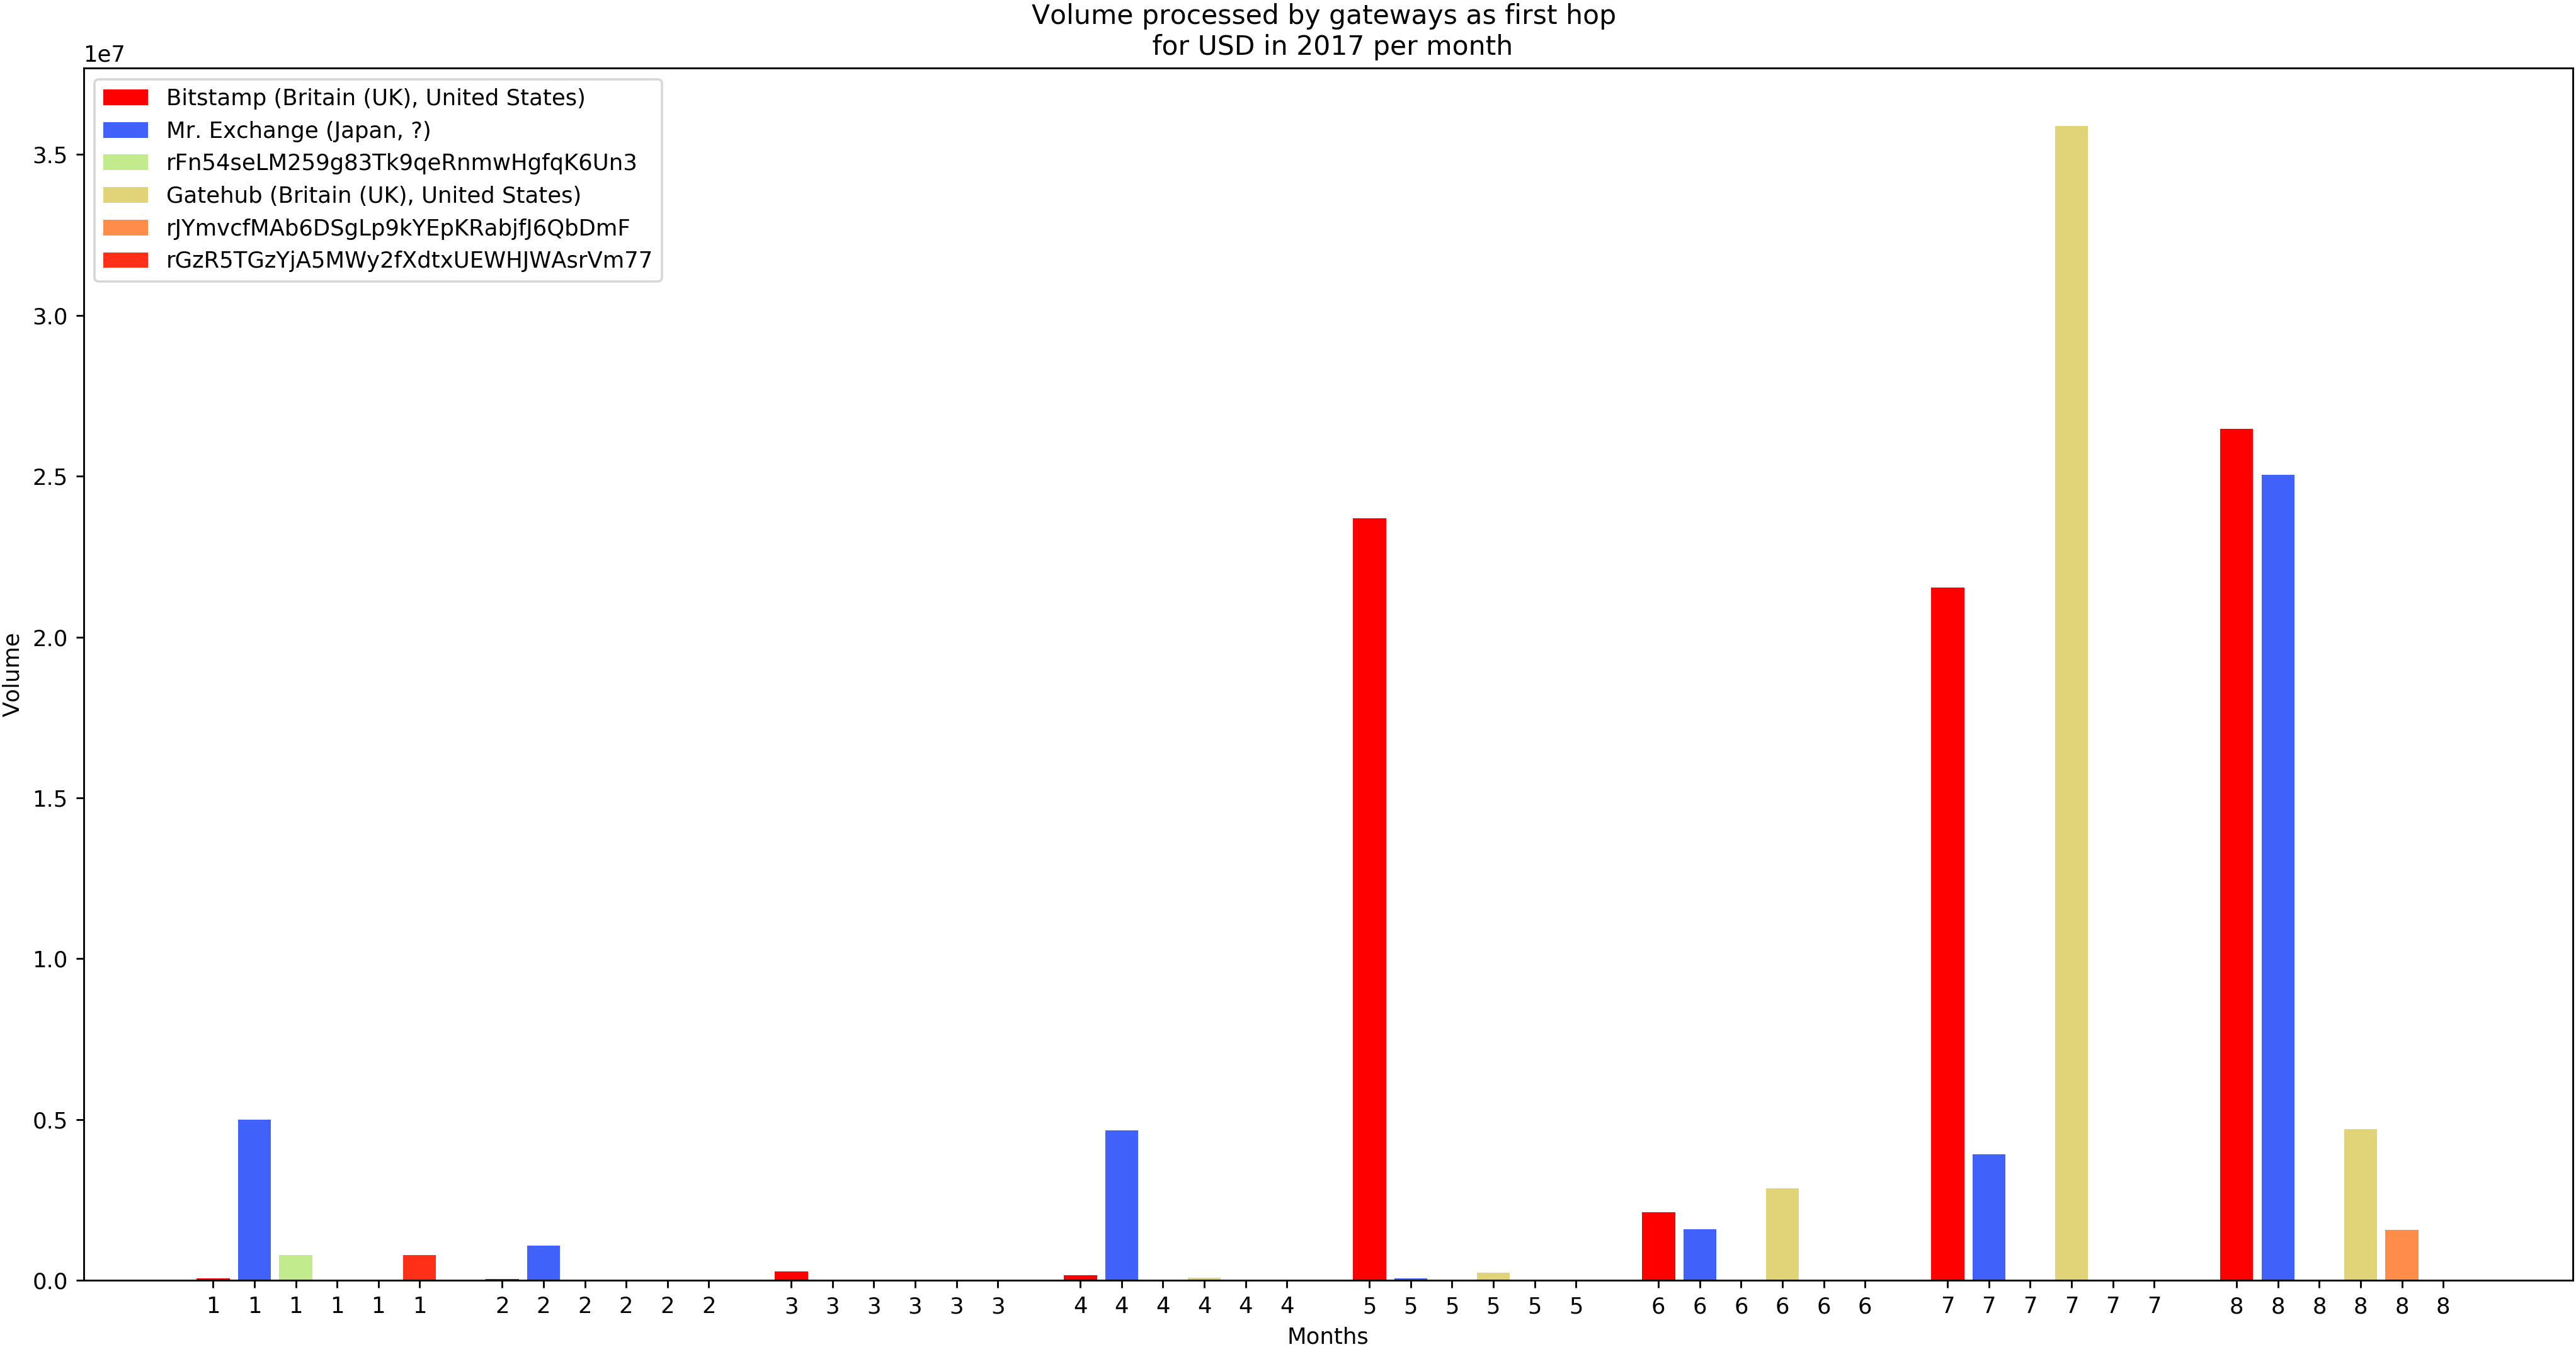
\includegraphics[width=1.375\textwidth]{volume_processed_by_gateways_as_first_hop_for_USD_in_2017_per_month.png}}
  \caption{Volume routed trough wallets as first hop for USD in 2017}
  \label{fig:first_hop_USD_volume}
\end{figure}

Figure \ref{fig:first_hop_USD_nb_txns}  (page 11) shows the number of transactions, with sender using USD, routed through each wallet and Figure \ref{fig:first_hop_USD_volume}  (on page 12) shows the same transactions but in terms of volume. On the x-axis, you can see numbers that represent the month of the year. There is one tick by wallet and by month. We see that the number of transaction increase over time, we can see this increase in the volume plot too but it seems let smooth. It is also interesting to notice the difference between the wallets that appears in Figure \ref{fig:first_hop_USD_nb_txns} and Figure \ref{fig:first_hop_USD_volume}. Some wallets are insignificant in terms of the number of transactions but appear in the volume graph. You can also see that for wallets that are gateways we showed their names and their respective fiscal and servers geographical positions (as in Figure \ref{fig:first_lap_hop_per_gateway}). We saw in this last figure that gateways seemed to specialized but remark here that none of the gateways for USD are fiscally situated in the USD. 
\vspace{\baselineskip}

\begin{figure}[h!]
  \makebox[\textwidth][c]{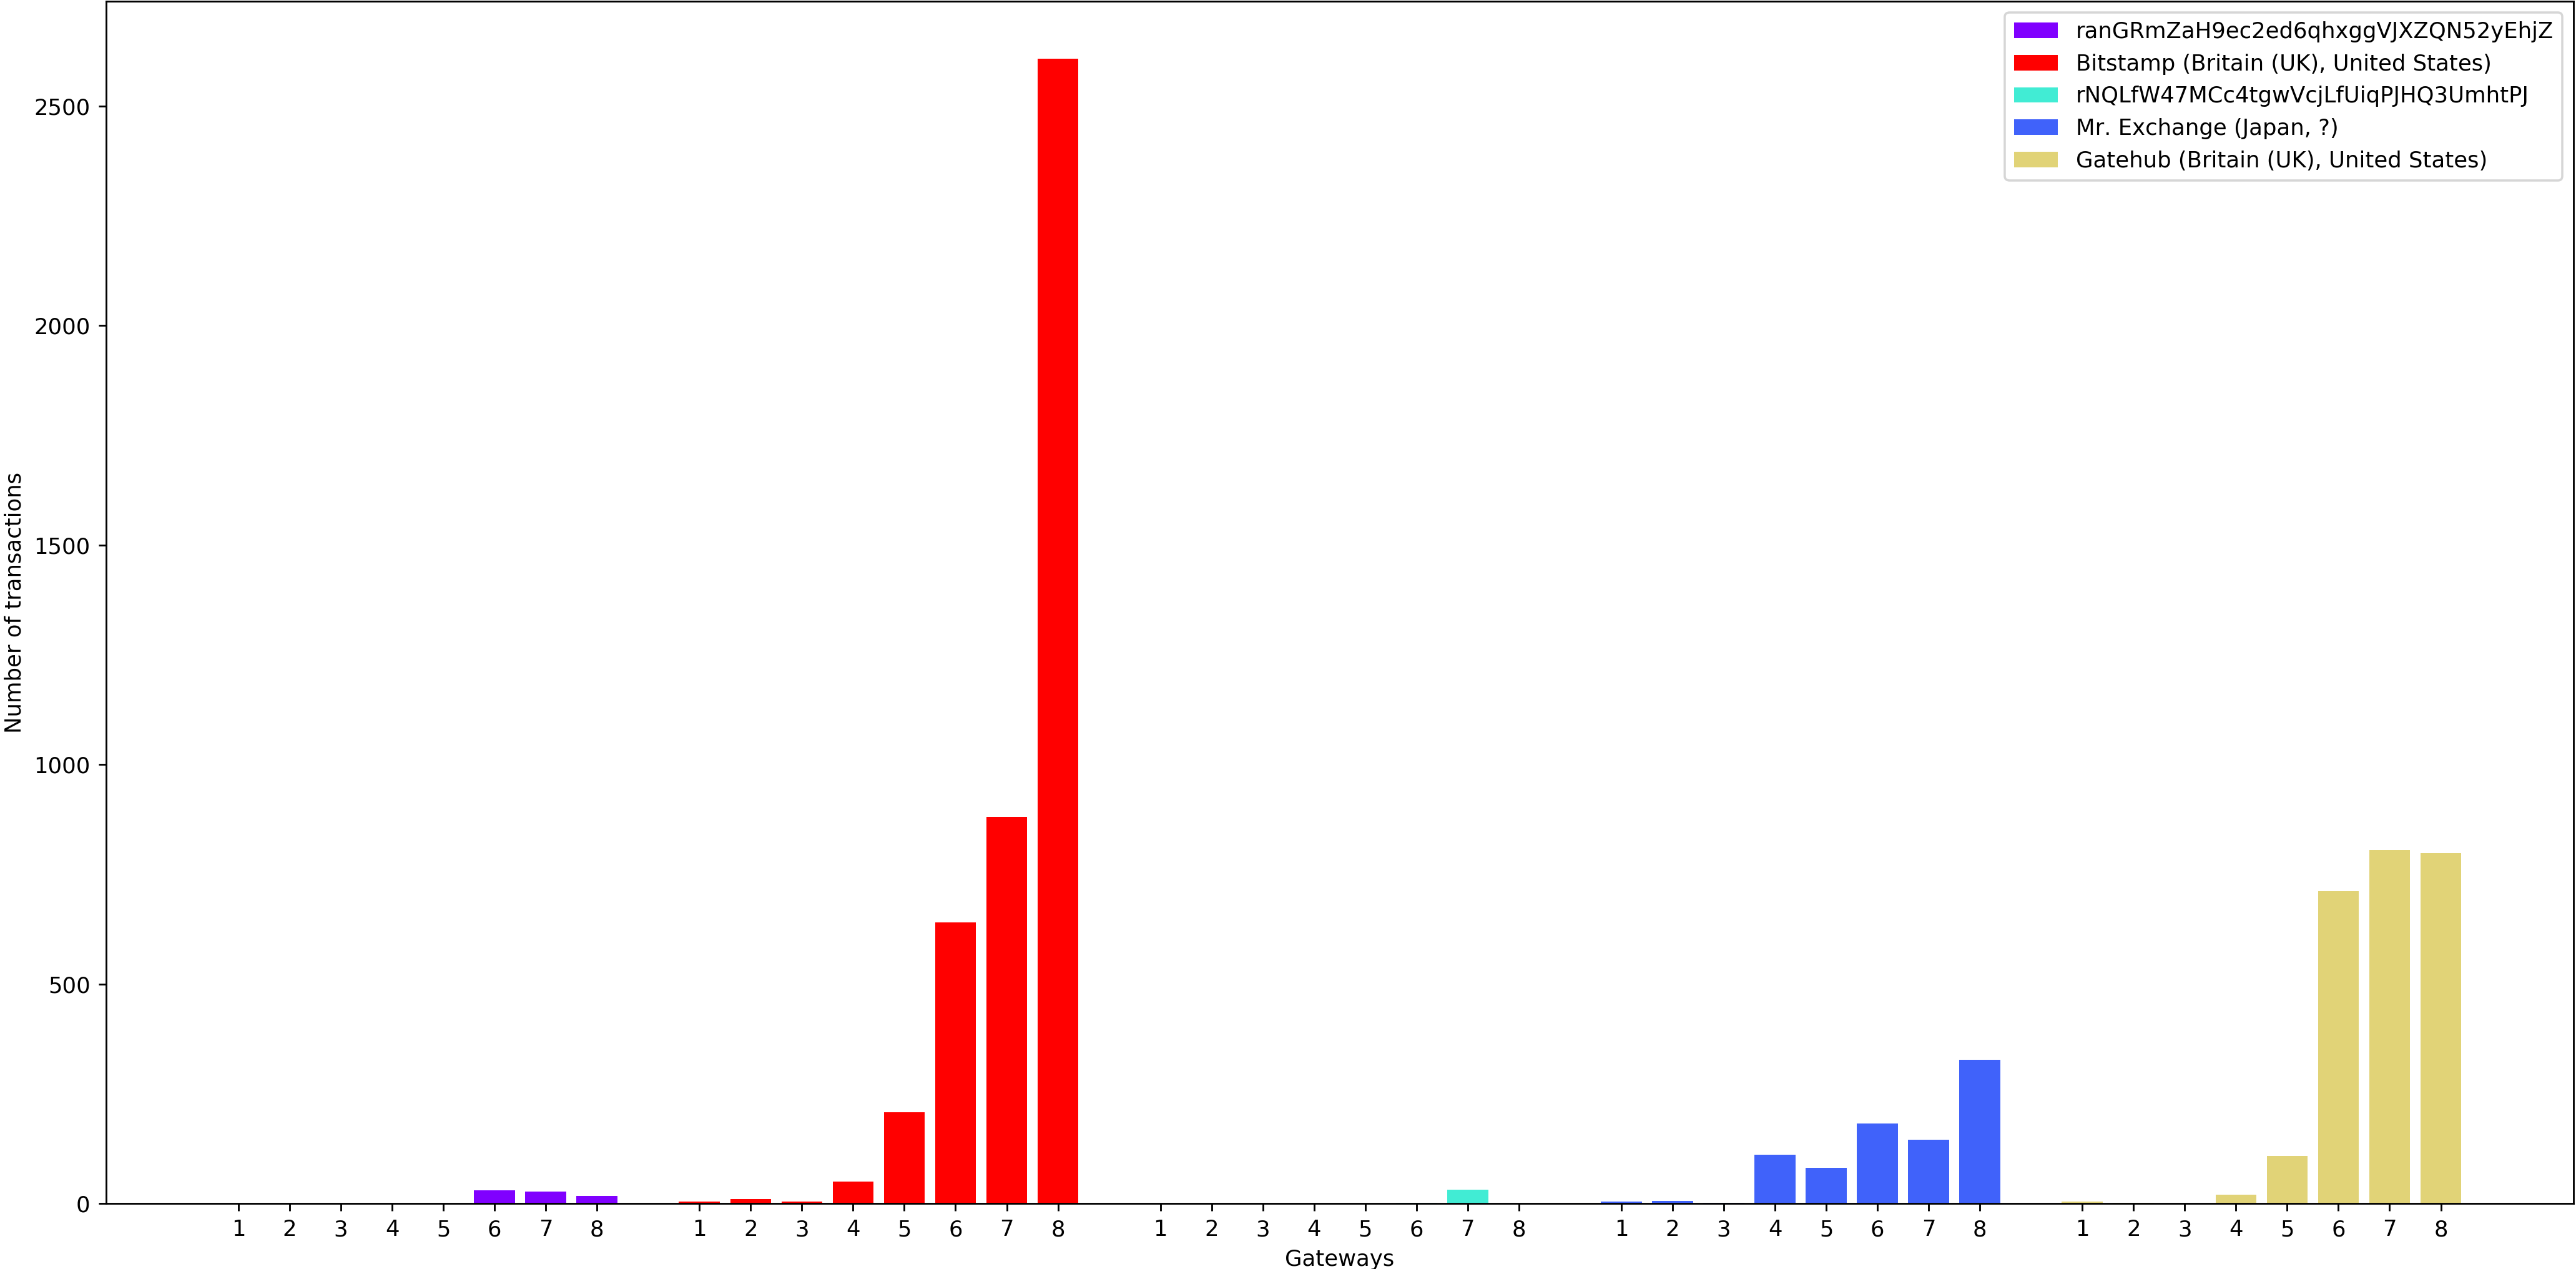
\includegraphics[width=1.375\textwidth]{number_of_transactions_processed_by_gateways_as_last_hop_for_USD_in_2017_per_gateway.png}}
  \caption{Number of transactions routed trough wallets as last hop for USD in 2017}
  \label{fig:last_hop_USD_nb_txns}
\end{figure}

\begin{figure}[h!]
  \makebox[\textwidth][c]{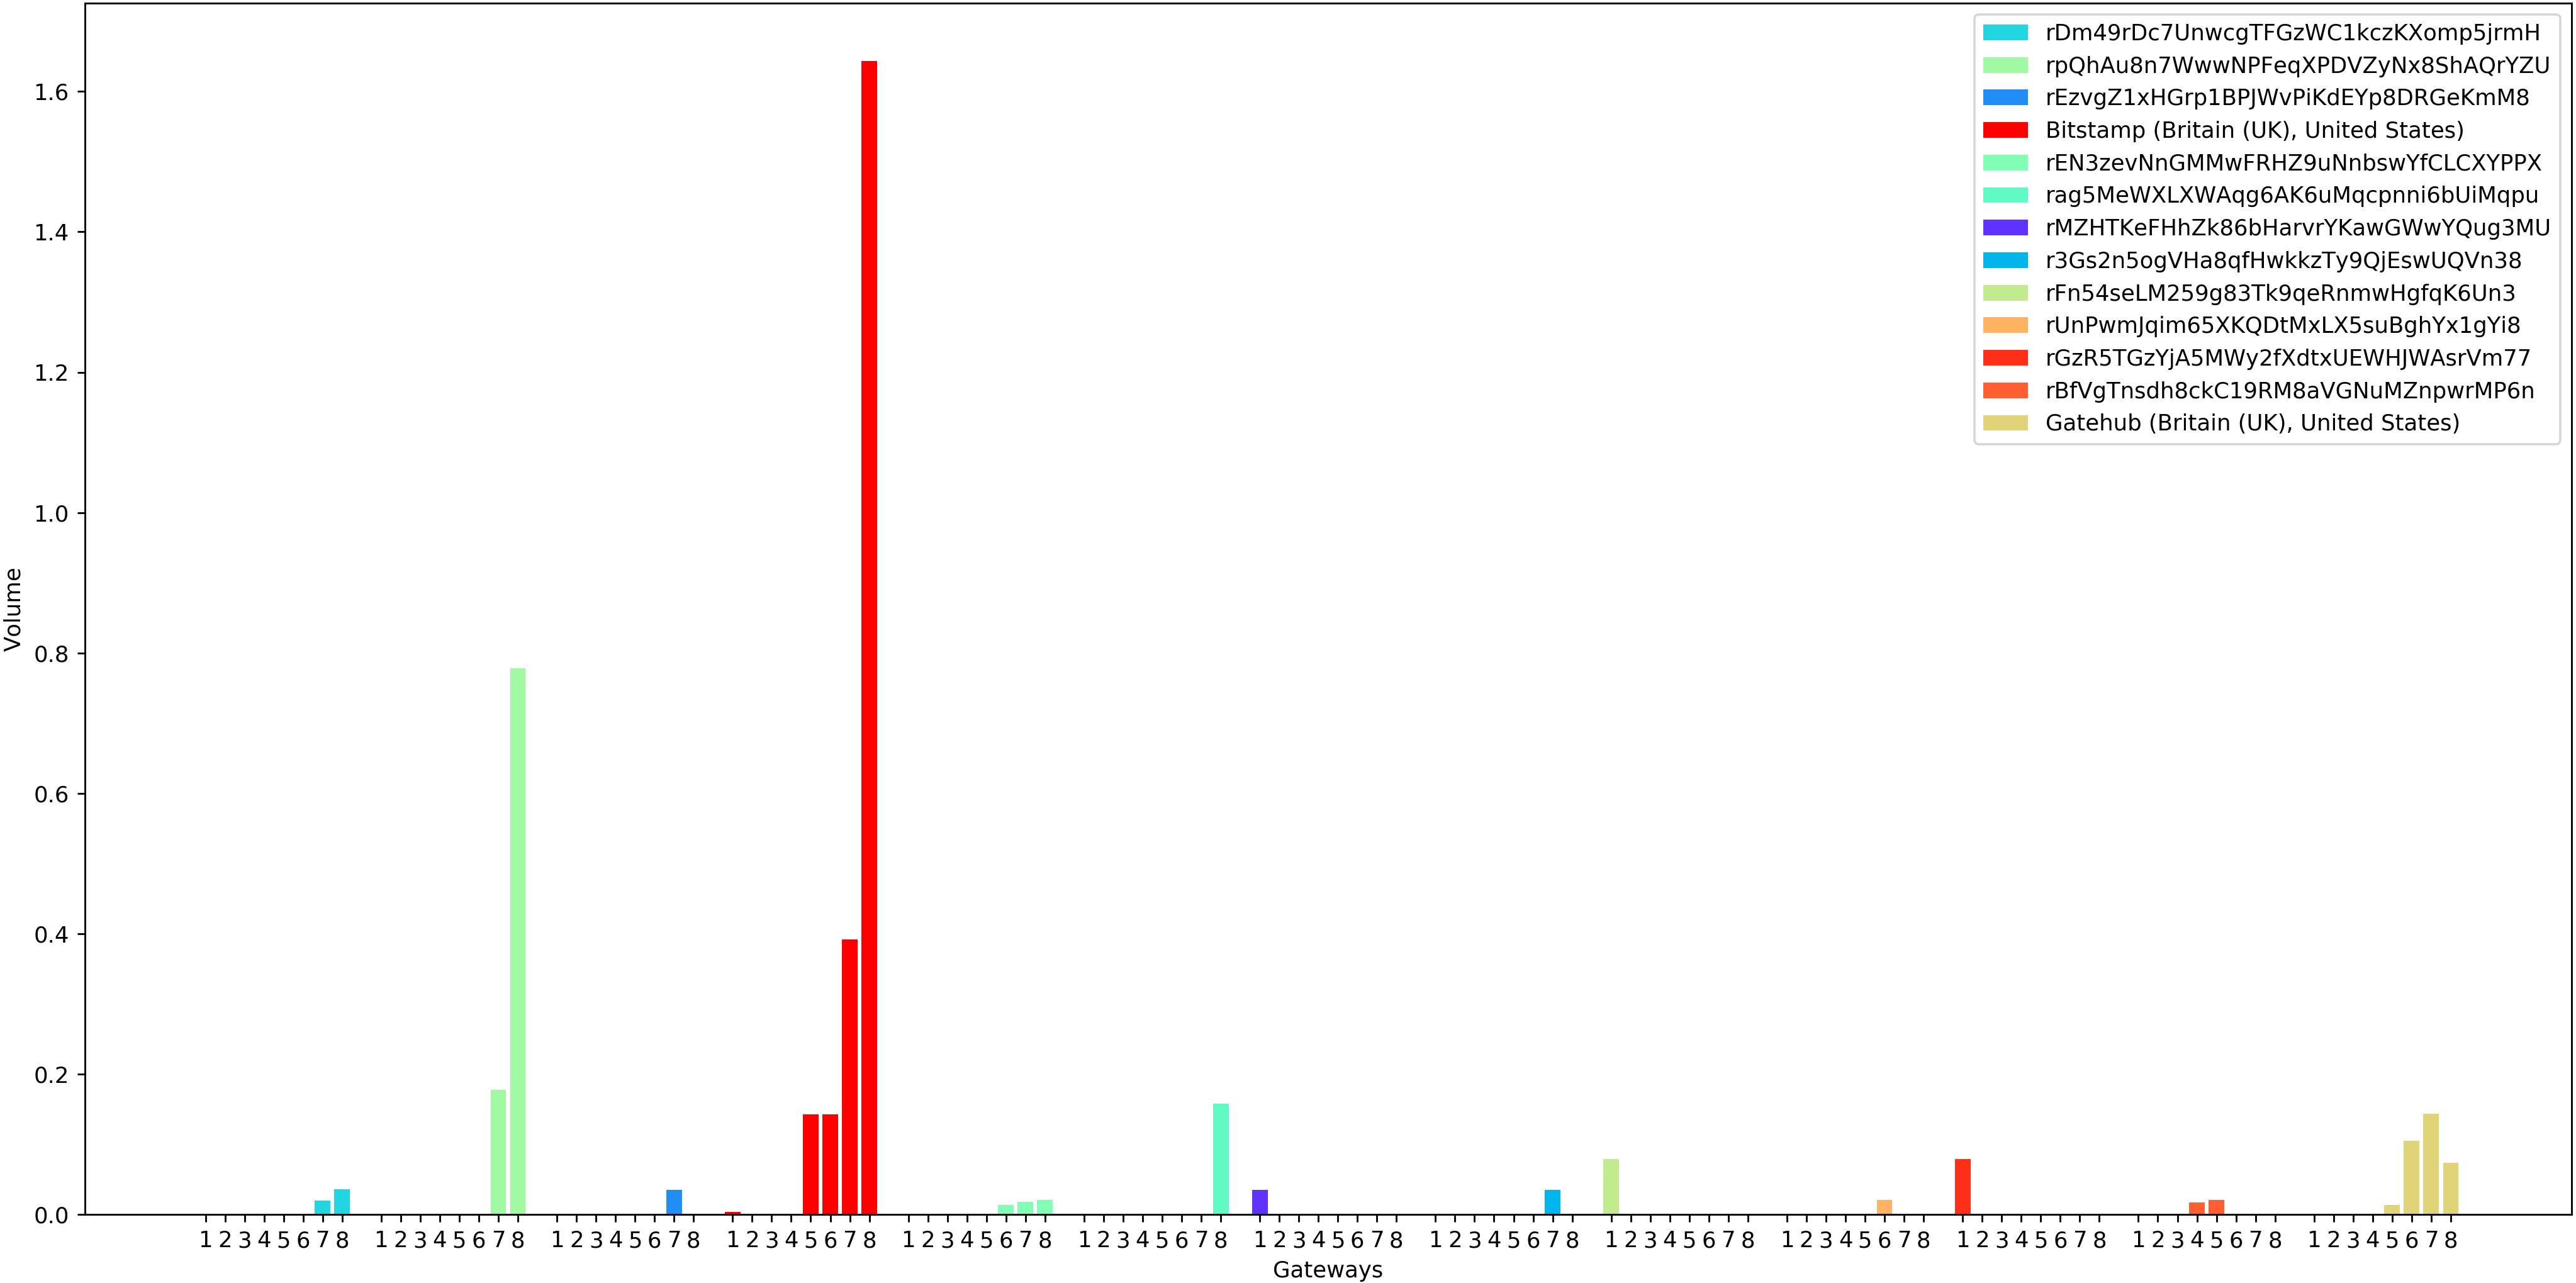
\includegraphics[width=1.375\textwidth]{volume_processed_by_gateways_as_last_hop_for_USD_in_2017_per_gateway.png}}
  \caption{Volume routed trough wallets as last hop for USD in 2017}
  \label{fig:last_hop_USD_volume}
\end{figure}
Let's now look as the same data but for last hops in USD over 2017. The x-axis of Figures \ref{fig:last_hop_USD_nb_txns} and \ref{fig:last_hop_USD_volume} (on page 13) represent also the time progression but instead of grouping by month as in Figures \ref{fig:first_hop_USD_nb_txns} and \ref{fig:first_hop_USD_volume} we group by gateway and for each gateway have the eight months. 

The results are similar to what we could get from the first hops. However this time there is much more wallets that are not known as gateways. We see that the gateway Bitstamp is the most popular wallet for first and last hop. For the last hop the gateway Mr. Exchange that does appear in the number of transactions plot is absent from the graph with the volume. In this graph, we have only gateways with their fiscal location outside of the United States. After looking at the plot for the other currencies, it seems that USD is the only currency to behave like this.
\vspace{\baselineskip}

In this subsection, we wanted to dig into the evolution of credit links. From what we see it seems that the most popular wallets, that turns out to be gateways, appears usually in each month over 2017. We can conclude that credit links seem quite regular for the wallets with high activity in the Ripple Network. However, we also found wallets, that are not gateways, which appears to have high activity. We didn't have time to investigate further on those wallets and this is left out as further work.
\newpage
\subsubsection{Looking at currencies}
Next step in our analysis of transaction locality. We looked at the sender and receiver currency pair and if there were any correlation. We expect to find here a lot of cross-currency payment in the Ripple Network. We looked at all transactions in our data and counted the number of transactions that correspond to each possible sender and receiver currency pairs.
\begin{figure}[h!]
    \centering
    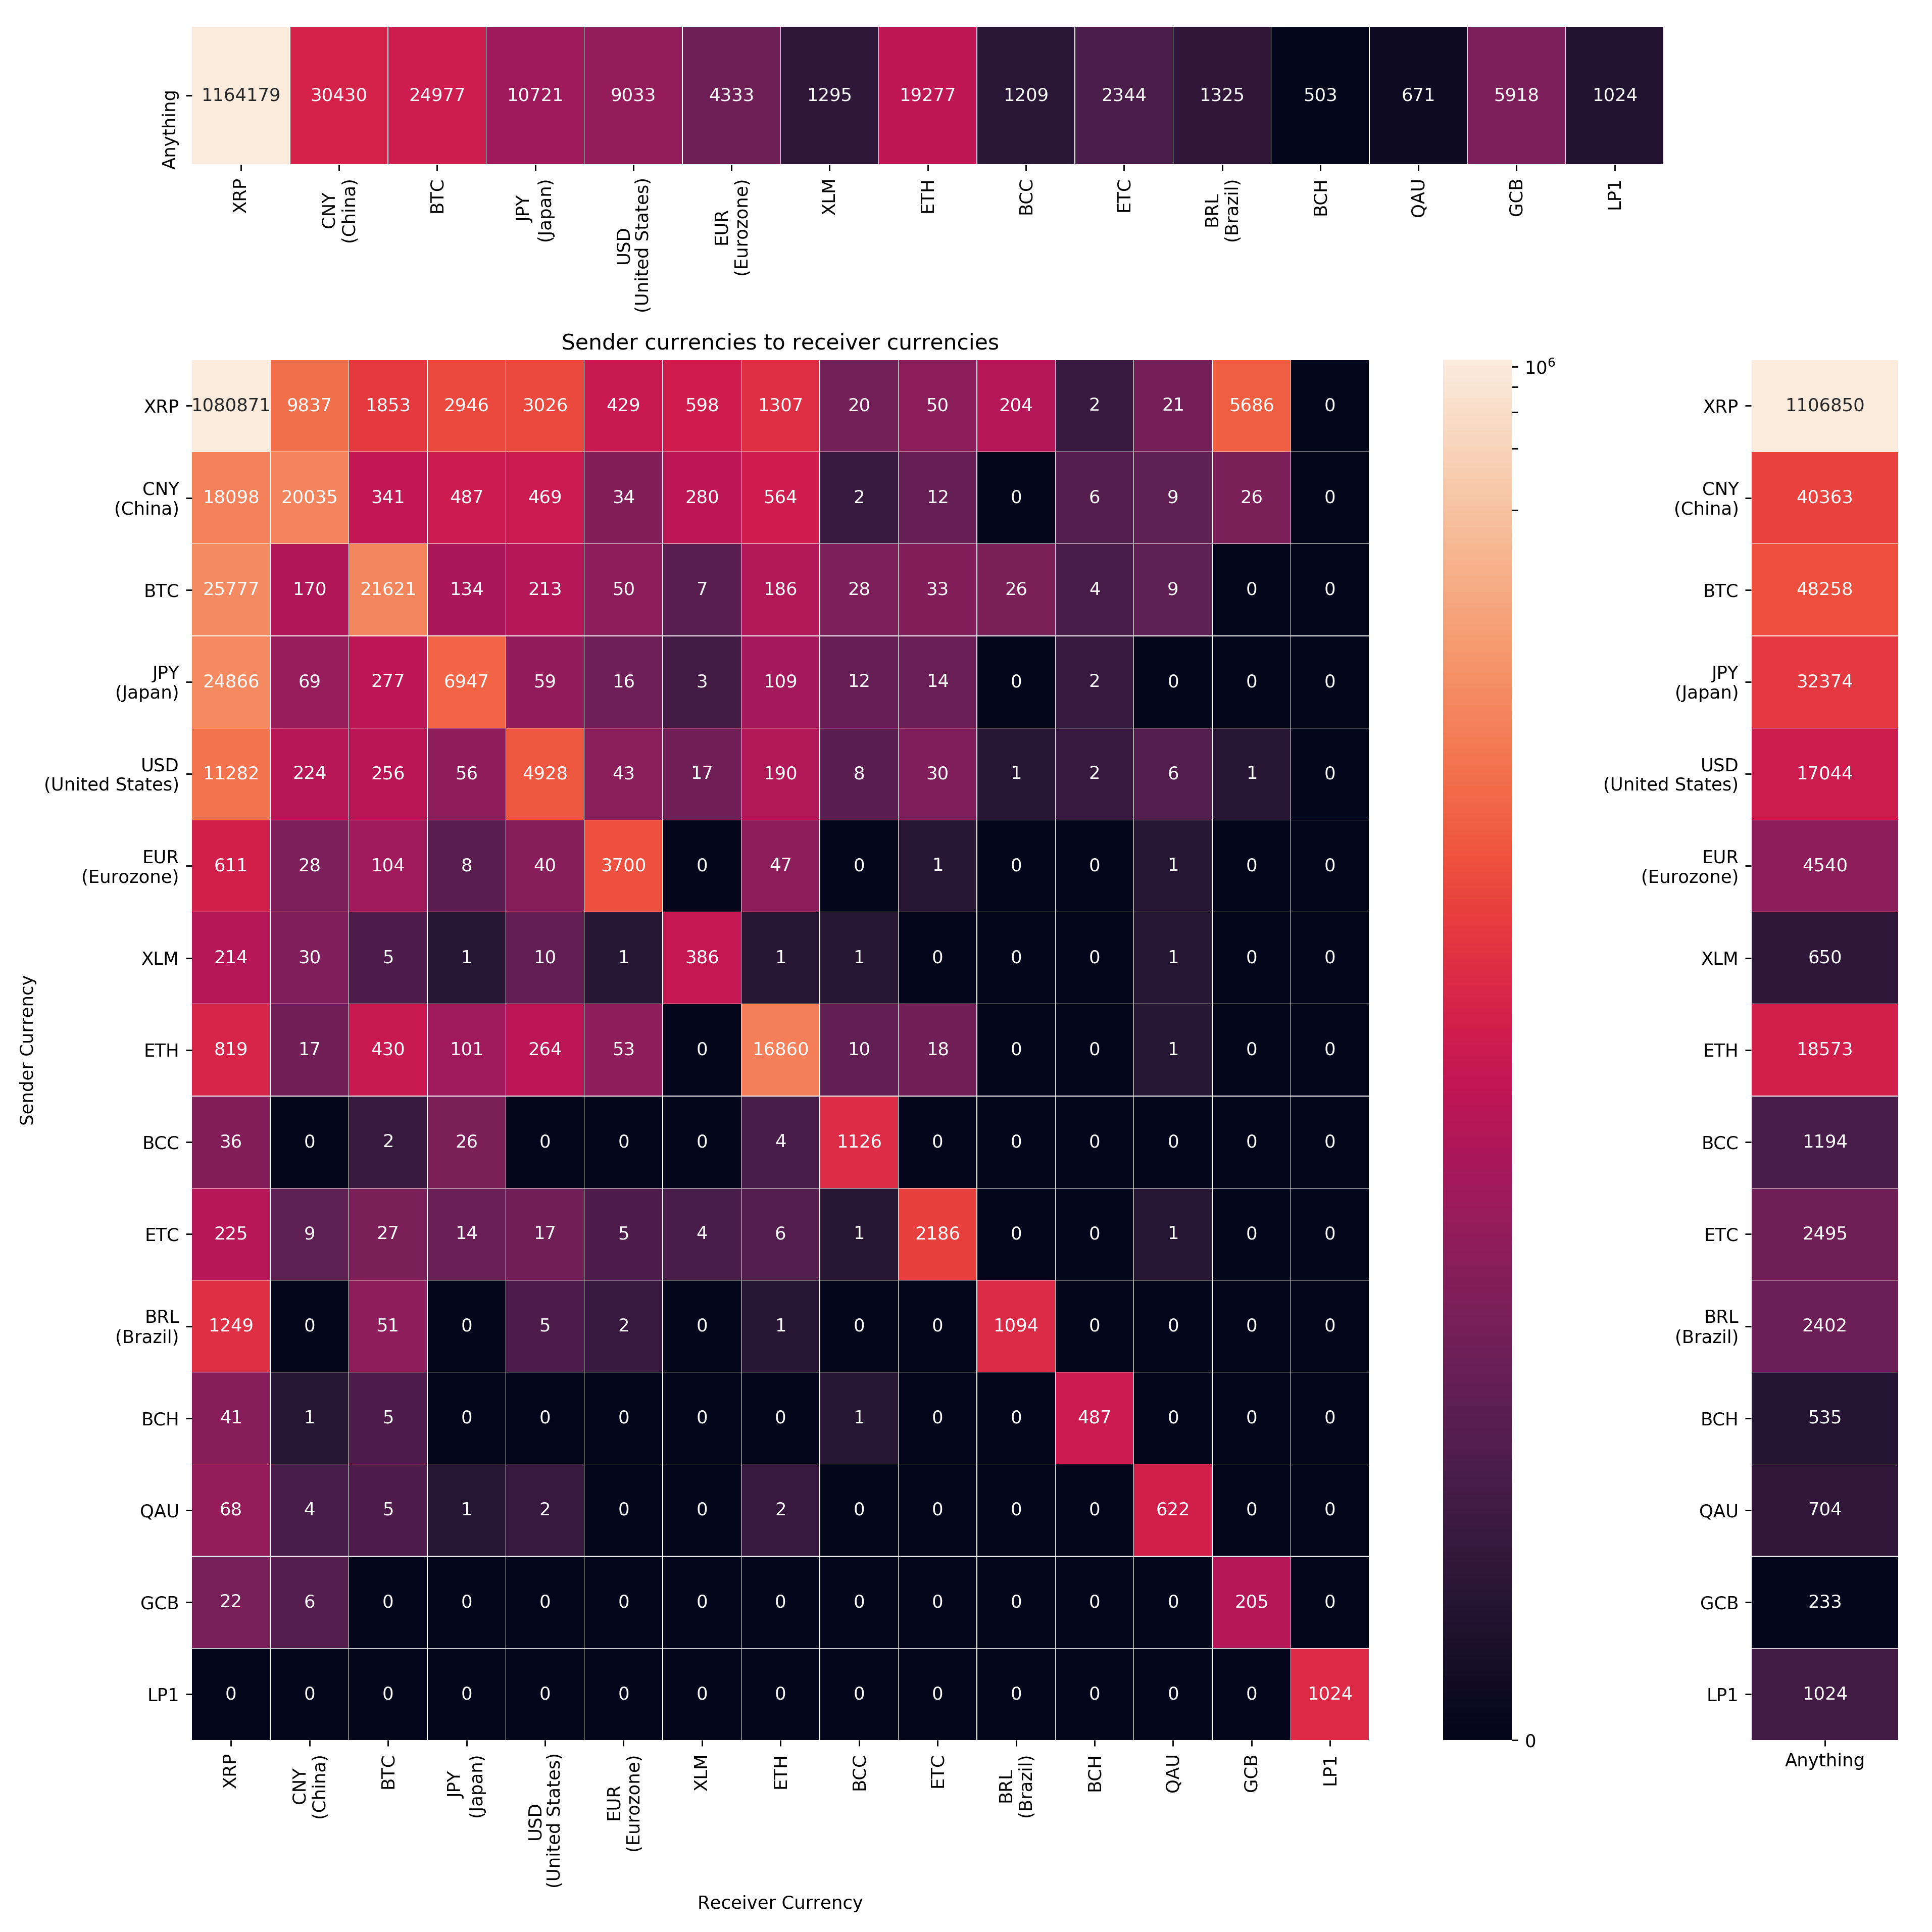
\includegraphics[width = \linewidth]{sender_to_receiver_heatmap.png}
    \caption{Sender Receiver Currency Paris in number of transactions}
    \label{fig:heatmapNbTxns}
\end{figure}
The heat-map in Figure \ref{fig:heatmapNbTxns} shows the result for the fifteen most popular currencies in terms of the number of transactions. The x and y-axis are currencies where the most popular currency is on the left (respectively on the top). Each cell of the heat-map shows the number of transactions for the corresponding sender/receiver pair. We used a logarithmic scale because when we first plotted this heat-map everything was black but the top left cell. This is because there are much more transactions that go from XRP to XRP than any other pair of currencies. Again what is important is not the actual numbers but the colors. The more bright a cell is then the more there are transactions for the corresponding currency pair. The diagonal pops out from this visualization, what does that mean? It means that there is a good amount of transactions that start and end in the same currency. Said differently, we don't have that many cross-currency payments. There are more same currency payments than cross-currency payments. We can also note that transaction from one currency to XRP seems to be quite common too, at least for the top 5 currencies without considering XRP. You might have noticed the top and left heat-maps. They represent respectively the number of transaction from any currency to a given currency and the number of transaction from a given currency to any currency.

We can also look at the heat-map for the same currencies but instead of the number of transactions, we have the volume in XRP.
\begin{figure}[h!]
    \centering
    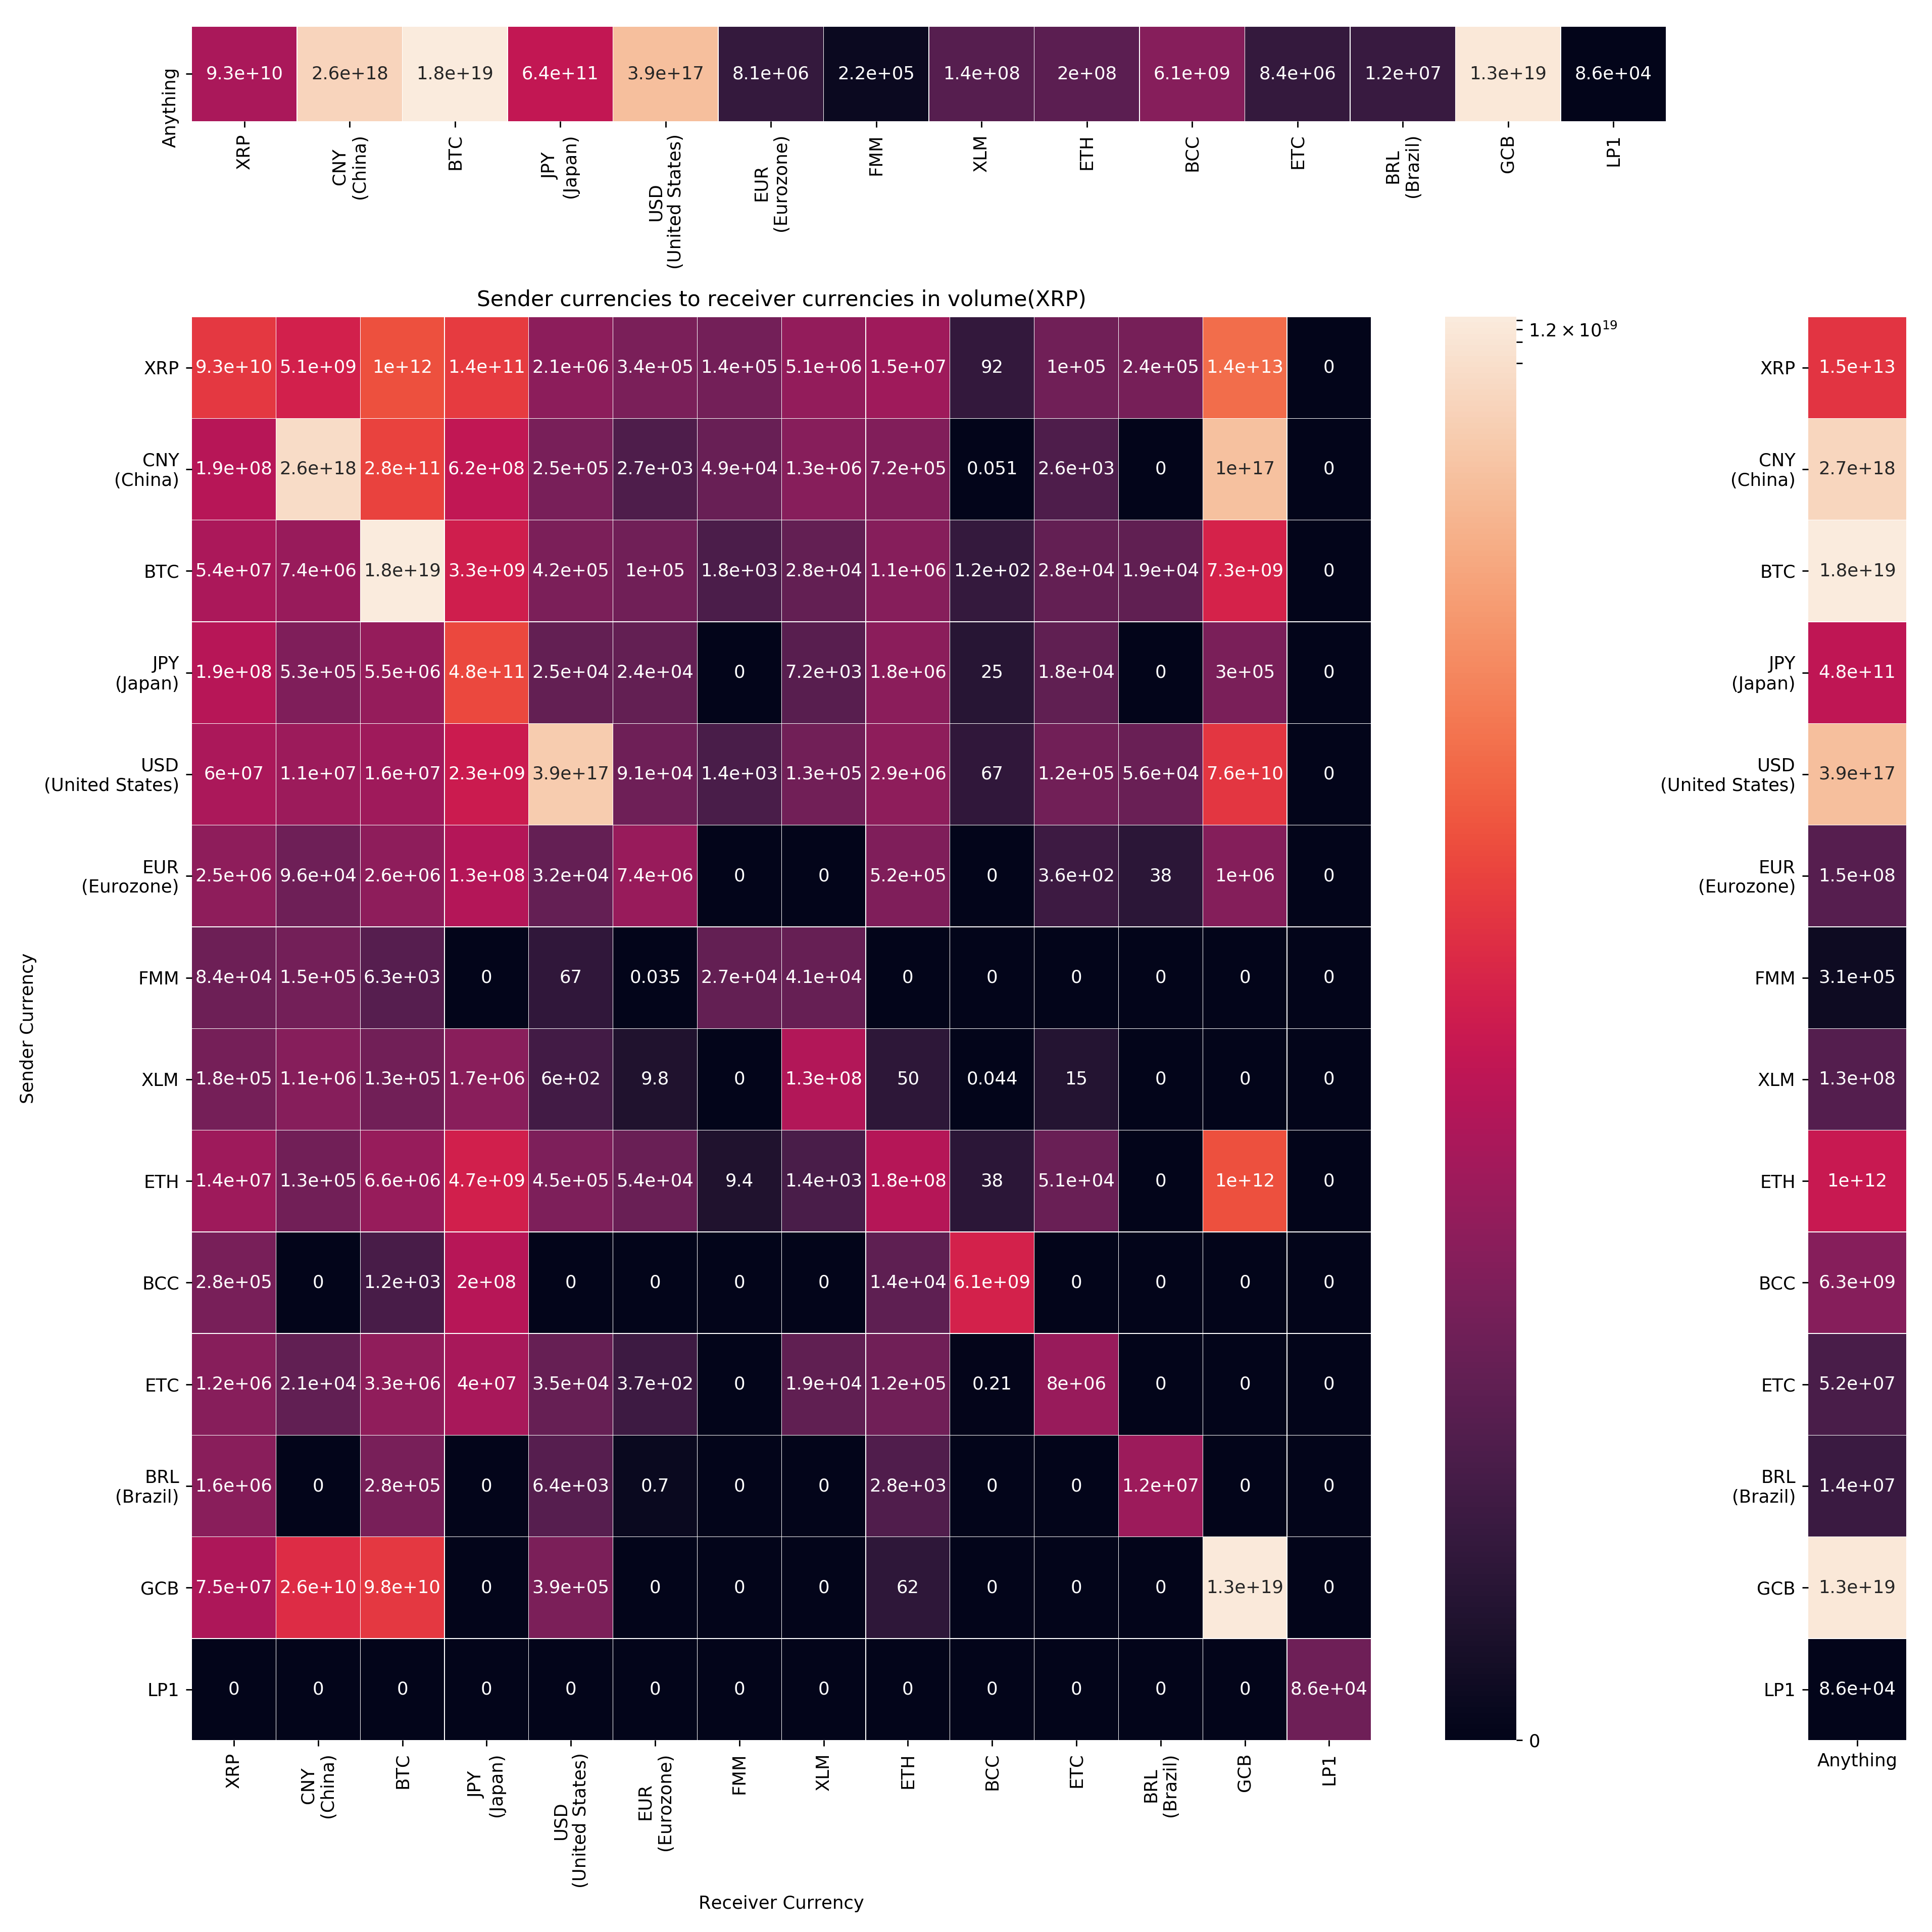
\includegraphics[width = \linewidth]{sender_to_receiver_heatmap_volume.png}
    \caption{Sender Receiver Currency Paris in volume (XRP)}
    \label{fig:heatmapVolume}
\end{figure}
 The heat-map in Figure \ref{fig:heatmapVolume} shows the result for the fifteen most popular currencies in terms of volume. The scale is also logarithmic. The results are quite similar to the previous ones. As for the number of transactions, the diagonal pops out from this visualization. Those results reinforce that there are a high number of transactions that start and end in the same currency. 